\definecolor{red}{rgb}{0.827,0.196,0.122}
\definecolor{orange}{rgb}{1.0,0.498,0.0}
\definecolor{olive}{rgb}{0.71,0.71,0.345}
\definecolor{green}{rgb}{0.118,0.490,0.216}
\definecolor{blue}{rgb}{0.447,0.624,0.812}

\chapter{Entwurf}
\label{chapter:design}
    Nachdem im vorangegangenem Kapitel die Anforderungen für das System spezifiziert wurden, soll in diesem Kapitel der Umsetzungsentwurf der verschiedenen Sichten dargestellt werden.
    Zunächst wird das dem System zugrundeliegende Datenmodell dargestellt.
    Darauffolgend wird das Design für die webbasierte Plattform erläutert.     
    
    \section{Datenmodell}
        \begin{figure}
            \centering
            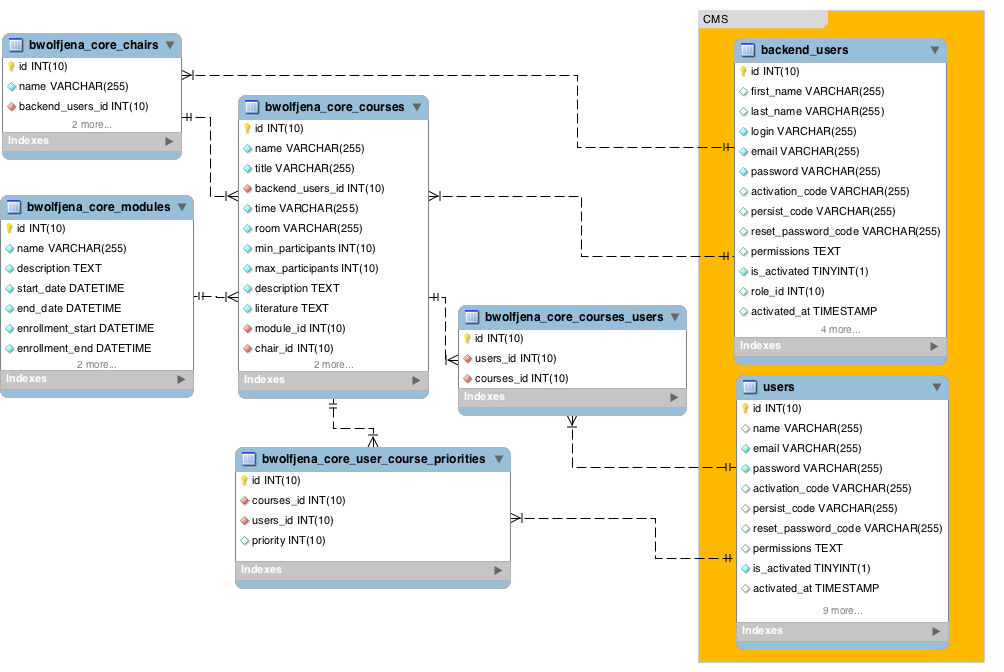
\includegraphics[width=1.0\textwidth]{./design/images/data-model.png}\par\vspace{1cm}
            \caption{Entwurf des Datenmodells. Farbcode für Spalten der Tabellen: Gelb Primärschlüssel, Rot Fremdschlüssel, Blau gewöhnliche Variable, Weiß nullable Variable}
            \label{fig:datamodel}
        \end{figure}
    
        Der Entwurf für das Datenmodell ist in Abbildung \ref{fig:datamodel} zu sehen.
        Es besteht aus sieben Tabellen.
        Die Tabelle \textit{bwolfjena\_core\_modules} beinhaltet die verschiedenen Empiriepraktika.
        Der Name Module für die Tabelle wurde gewählt, da das System bei Bedarf auch auf andere ausgewählte Module als das Empiriepraktikum erweitert werden kann.
        
        In der Tabelle \textit{bwolfjena\_core\_courses} sind die verschiedenen Kurse gespeichert.
        Ein Kurs gehört immer zu einem bestimmten Modul beziehungsweise einem Empiriepraktikum.
        Um das abzubilden, ist für jeden Kurs mittels eines Fremdschlüssels das Empiriepraktikum, zu dem er gehört, gespeichert.
        
        Ein Kurs wird immer von einem Lehrstuhl angeboten, die in der Tabelle \textit{bwolfjena\_core\_chairs} abgelegt sind.
        Auch auf diese Tabelle existiert wieder ein entsprechender Fremdschlüssel in \textit{bwolfjena\_core\_courses}. 
        
        Alle angemeldeten Studenten werden in der Tabelle \textit{users} gespeichert.
        Jeder der Studenten hat eine Präferenzliste.
        Die Einträge der Präferenzliste für jeden Studenten und jeden Kurs werden in Tabelle \textit{bwolfjena\_core\_priorities} gespeichert.
        Dementsprechend beinhaltet \textit{bwolfjena\_core\_priorities} Fremdschlüssel von \textit{users} und \textit{bwolfjena\_core\_courses}.
        
        In der Tabelle \textit{bwolfjena\_core\_users} ist abgelegt, welcher Student welchem Kurs zu geteilt wurde.
        Aus diesem Grund beinhaltet \textit{bwolfjena\_core\_users} Fremdschlüssel auf \textit{bwolfjena\_core\_courses} und \textit{users}. 
        
        Die letzte Tabelle \textit{backend\_users} beinhaltet die Backendbenutzer.
        Damit sind die Dozenten und Administratoren gemeint.
        In \textit{bwolfjena\_core\_courses} ist ein Fremdschlüssel für die Backendbenutzer gespeichert, um den Dozenten anzugeben, der den Kurs leitet.
        Auch die Tabelle \textit{bwolfjena\_core\_chairs} hat einen Fremdschlüssel zu der Tabelle \textit{backend\_users}, um den Lehrstuhlinhaber anzugeben.
        
        Neben den beschriebenen Fremdschlüsseln existieren für die Einträge in jeder Tabelle IDs als Primärschlüssel.
        Die weiteren Spalten der Tabellen sind entsprechend den Anforderung aus Kapitel \ref{chapter:requirements} gewählt.
        
        
        
    
    \section{Design}
        Für den Desing-Entwurf der Seite wurden Mock-Ups erstellt, die den groben Aufbau der Website mit den entsprechenden Funktionen zeigen. 
        Im folgenden werden diese Mock-Ups für das sogenannte Frontend, also aus Sicht der Studenten, und für das Backend, die Sicht der Dozenten beziehungsweise der Administratoren, vorgestellt.
        Dabei gilt der in Tabelle \ref{tab:Farbcode} angegebene Farbcode für die verschiedenen Elemente der Mock-Ups.
        \begin{table}
            \centering
            \begin{tabular}{l c| l}
                \cellcolor{red} & & Eingabefeld\\
                \cellcolor{orange} & & Button\\
                \cellcolor{olive} & & Drag\&Drop-Element\\
                \cellcolor{green} & & Textfeld\\
                \cellcolor{blue} & & Optisches Element
            \end{tabular}
            \caption{Farbcode der Mock-Ups}
            \label{tab:Farbcode}
        \end{table}
    
        \subsection{Frontend}
            Wie in Kapitel \ref{chapter:requirements} bereits ausgeführt, sollen die Studenten zunächst eine Registrierungs- bzw. Login-Oberfläche sehen.
            Jedoch sollen die verschiedenen Kurse auch ohne eine Anmeldung einsehbar sein.
            \begin{figure}[t]
            	\centering
            	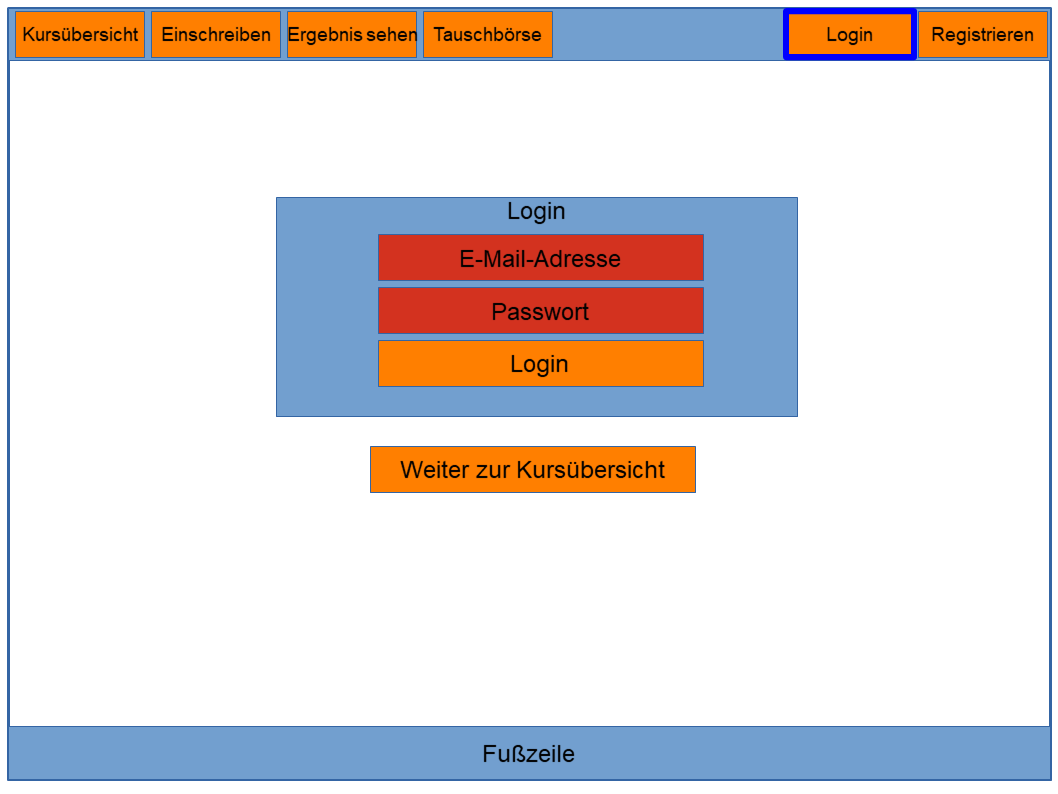
\includegraphics[width=0.6\textwidth]{./design/images/MockUpsFrontend/frontendLogin.png}
            	\caption{Entwurf für die Login-Oberfläche}
            	\label{fig:mockupLoginFrontend}
            \end{figure}   
        
            In Abbildung \ref{fig:mockupLoginFrontend} werden beide Anforderungen umgesetzt.
            Zum einen die Login-Oberfläche, in der in zwei Textfeldern Benutzername und Passwort für einen erfolgreichen Login eingetragen werden müssen, zum anderen die direkte Weiterleitung zur Kursübersicht als einfacher Knopf darunter.

            Die Kopfzeile umfasst einige Reiter.
            So kann mithilfe der Kopfzeile auf die verschiedenen Funktionen des Frontends gewechselt werden. 
            Dazu zählen die Kursübersicht, die Erstellung der Präferenzliste, das Einsehen der Verteilungsergebnisse, sowie das Tauschen von Kursen.
            Außer der Navigation auf die Kursübersicht sind diese jedoch erst nach einer erfolgreiche Anmeldung funktional.
            Ohne eine Anmeldung wird der Benutzer wieder auf die Loginoberfläche verwiesen.
            In der Kopfzeile soll auch eine Schaltfläche zum erstmaligen Registrieren im System sein.
            Die Registrierungsseite soll wie die der strukturell wie der Login aussehen (\ref{fig:mockupRegistrationFrontend}).
            Sobald ein Benutzer sich erfolgreich angemeldet hat, soll der Schalter zum Anmelden in der Kopfzeile gegen einen Abmelden-Knopf ausgetauscht werden.
%            Auch eine Anzeige, ab wann das Ende der Einschreibungs- und Tauschphase erreicht ist.
			Auf allen weiteren Seiten des Frontends soll die Kopfzeile die gleichen Funktionen und das gleiche Aussehen haben, der Registieren-Knopf entfällt jedoch, sobald die Anmeldung erfolgt ist.
            Die Fußzeile soll weitere allgemeine Informationen bereitstellen, sofern diese von Nöten sein sollten, aber vor allem als optischer Abschluss der Seite dienen.
            Auch sie soll auf alle folgenden Seiten übernommen werden.
			
			\begin{figure}[t]
				\centering
				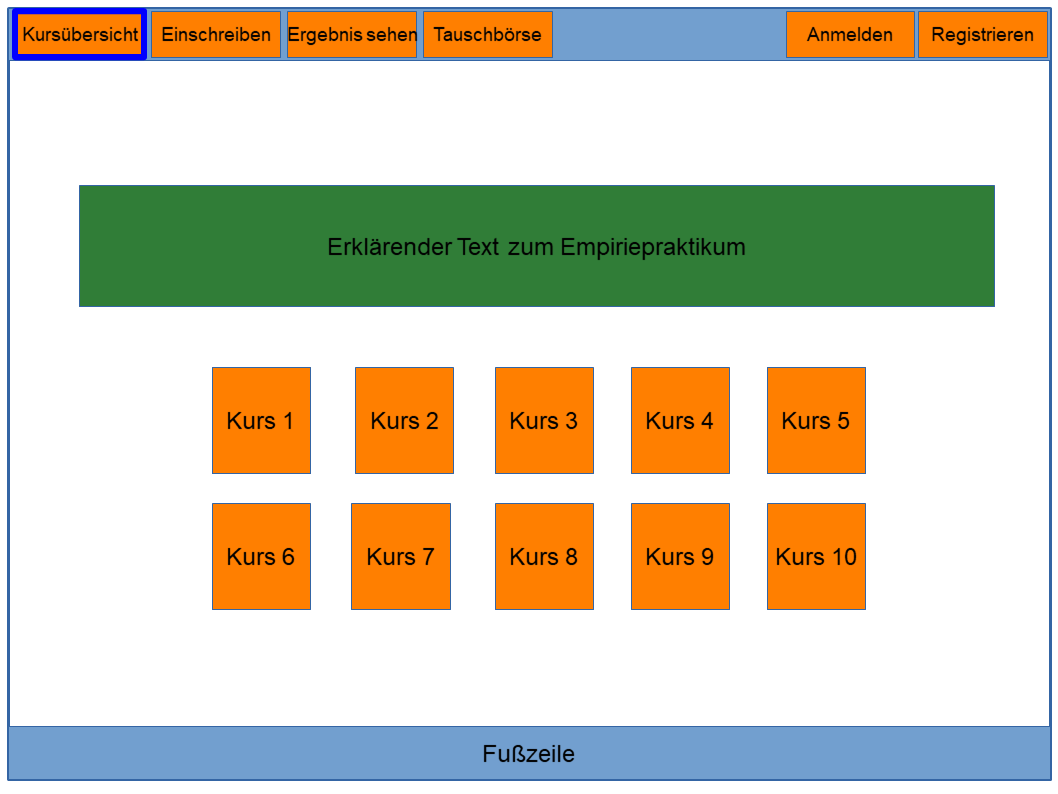
\includegraphics[width=0.6\textwidth]{./design/images/MockUpsFrontend/frontendCourses.png}
				\caption{Entwurf für die Kursübersicht}
				\label{fig:mockupCoursesFrontend}
			\end{figure}
			
			In Abbildung \ref{fig:mockupCoursesFrontend} ist die Seite für die Kursübersicht zu sehen.
            Unter der Kopfzeile folgt eine textuelle Erklärung des Ablaufs des Empiriepraktikums und der für die Studenten relevanten Schritte, um sich erfolgreich für die Kurse einzuschreiben.
            Die verschiedenen Kurse werden darunter jeweils mit einer kurzen Beschreibung angezeigt.
            Durch einen Klick auf ein Kursfeld, sollen sich die detaillierten Informationen zu dem Kurs einsehen lassen.
            Das Design hierfür ist in Abbildung \ref{fig:mockupDetailsFrontend} zu sehen und bedarf keiner weiteren Erläuterung.
            
            \begin{figure}[t]
            	\centering
            	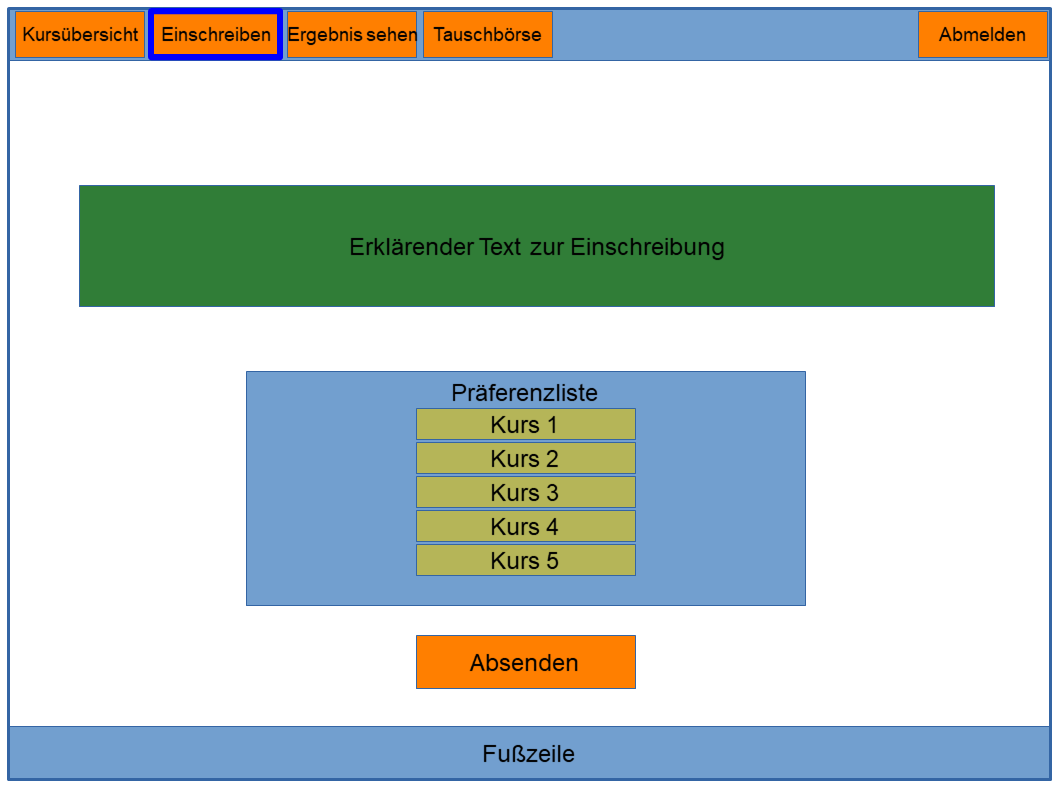
\includegraphics[width=0.6\textwidth]{./design/images/MockUpsFrontend/frontendPreferences.png}
            	\caption{Entwurf für die Einschreibungs-Oberfläche}
            	\label{fig:mockupPreferencesFrontend}
            \end{figure}
            
            Die Seite für die Einschreibung in die Kurse soll wie in Abbildung \ref{fig:mockupPreferencesFrontend} gestaltet sein.
            Wieder bilden Kopfzeile und Fußzeile den Rahmen der Seite.
            Unter der Kopfzeile befindet sich auch hier eine kurze Erklärung, wie man die Präferenzliste genau erstellt.
            Das Erstellen soll im Feld \textit{Präferenzliste} über ein ''Drag\&Drop''-System vorgenommen werden und über den Knopf \textit{Absenden} fixiert werden können.
            
            Nachdem die Verteilung auf die Kurse vorgenommen wurde, sollen die Benutzer unter dem Reiter Ergebnisübersicht die Resultate einsehen können.
            Der einfache Entwurf ist im Anhang \ref{chapter:appendix} in Abbildung \ref{fig:mockupResultsFrontend} zu sehen.
            
            Unter dem Reiter \textit{Tauschbörse} soll die in Kapitel \ref{chapter:requirements} genannte Tauschmöglichkeit für Studenten realisiert sein.
            Die Struktur der Seite gleicht dem der Kursübersicht.
            Unter einer Information in welchem Kurs man sich befindet und wie die Tauschfunktionen zu benutzten sind, finden sich die verschiedenen Kurse, genauso wie in der Kursübersicht.
            Der Kurs, dem man zugeteilt ist, erscheint ausgegraut oder auf eine andere Art und Weise markiert.
            
            \begin{figure}[t]
            	\centering
            	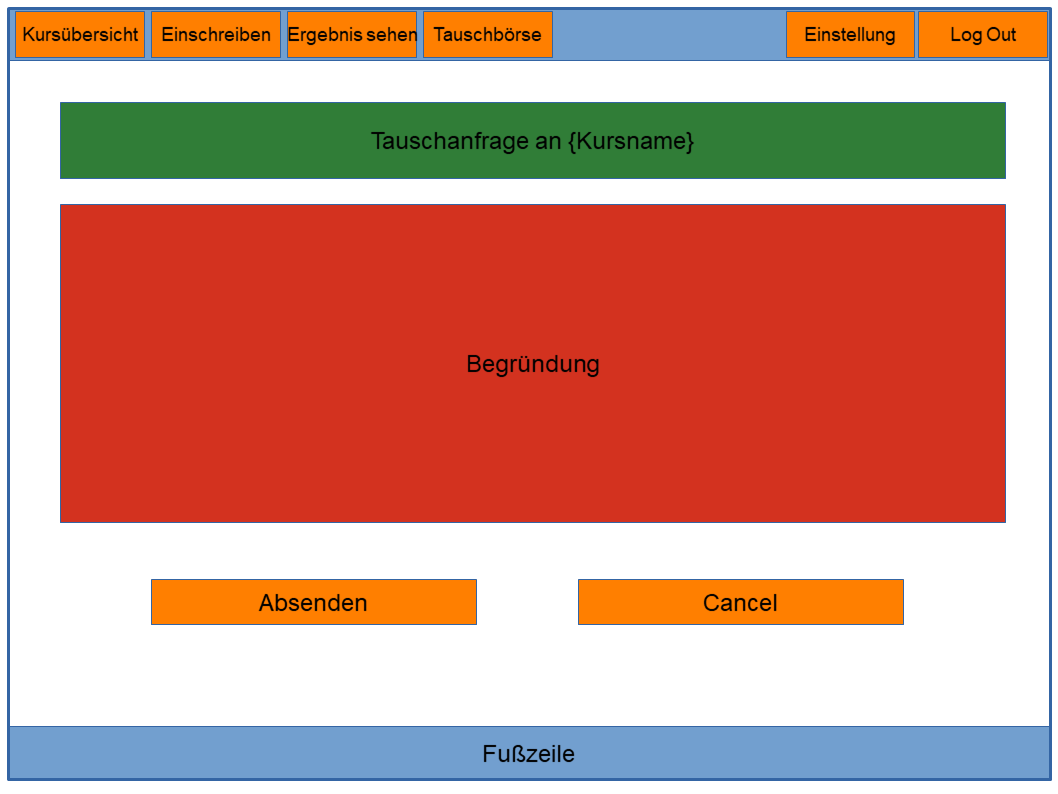
\includegraphics[width=0.6\textwidth]{./design/images/MockUpsFrontend/frontendSwap2.png}
            	\caption{Entwurf für die Tauschanfrage}
            	\label{fig:mockupResultsSwap2}
            \end{figure}
            
            Durch einen Klick auf den Kurs mit dem man Tauschen möchte, öffnet sich die in Abbildung \ref{fig:mockupResultsSwap2} gezeigt Seite.
            Hier kann in dem Textfeld \textit{Begründung} eine Begründung für den Tausch angegeben werden.
            Mit der Schaltfläche \textit{Absenden} kann die Tauschanfrage abgeschickt werden, mit \textit{Abbrechen} gelangt der Benutzer wieder auf die vorherige Ansicht der Tauschbörse.
            
            
            
        
            
            
    
        \subsection{Backend}
	        Im Folgenden werden die wichtigsten Mockups für Administratoren und Dozenten vorgestellt.
	        Für beide Sichten gibt es wieder eine Kopf- und eine Fußzeile.
	        Die Kopfzeile für die Administratoren umfasst zunächst einen Reiter \textit{Verwalten}, in dem Kurse, Module und Lehrstühle angelegt werden können.
	        Des Weiteren gibt es den Reiter \textit{Benutzer}, unter dem alle Benutzer des Systems verwaltet werden können.
	        Unter dem Reiter \textit{Verteilungsalgorithmus} können die Administratoren den Verteilungsalgorithmus starten und sich die Ergebnisse anzeigen lassen.
	        Zusätzlich gibt es noch eine Seitenleiste, in der unter dem jeweiligen Reiter weitere Optionen zur Verfügung stehen.
        	
        	\begin{figure}[t]
        		\centering
        		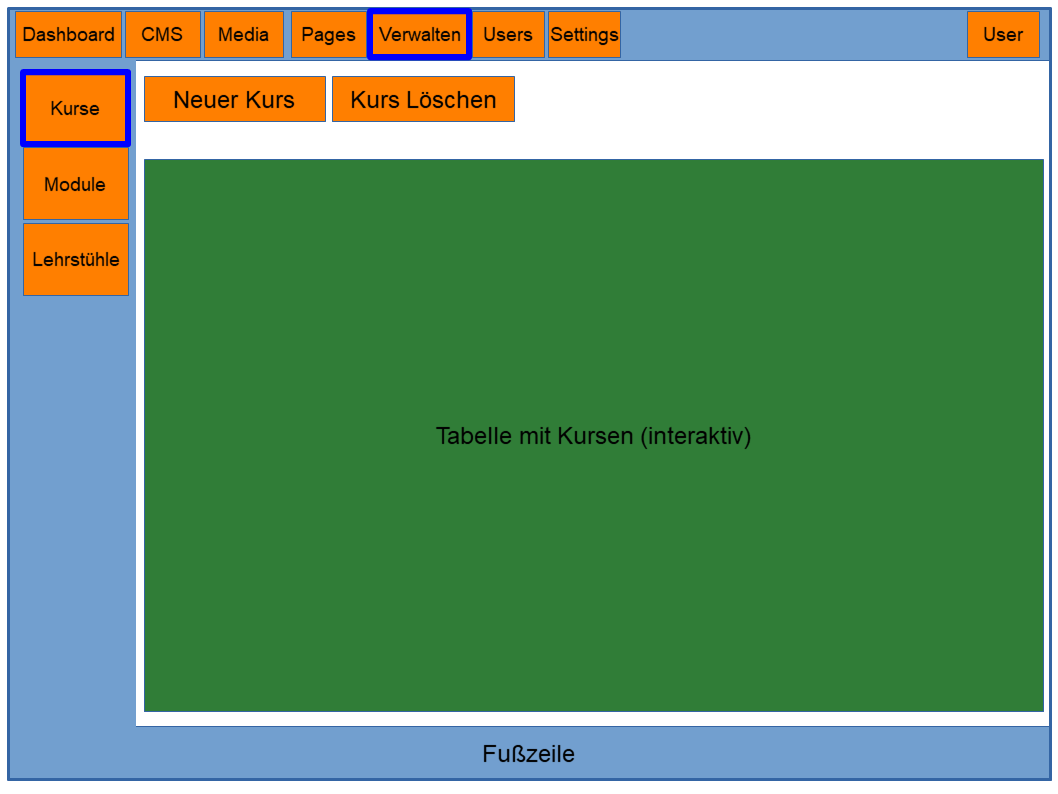
\includegraphics[width=0.6\textwidth]{./design/images/MockUpsBackend/backendManageCourses.png}
        		\caption{Entwurf für das Verwalten der Kurse}
        		\label{fig:mockupManageCourses}
        	\end{figure}
        	
        	In Abbildung \ref{fig:mockupManageCourses} ist beispielhaft für den Reiter Verwaltung, die der Kursverwaltung zu sehen.
        	Mithilfe der Seitenleiste am linken Rand, kann zwischen dem Verwalten von Kursen, Modulen (Praktika) und Lehrstühlen gewechselt werden.
        	Alle Vorhandenen Kurse (bzw. Module oder Lehrstühle) werden in einer Tabelle angezeigt.
        	Mit den beiden Schaltflächen am oberen Rand der Tabelle kann ein neuer Eintrag in der jeweiligen Tabelle erstellt, bzw. ein vorhandener Eintrag gelöscht werden.
        	Die Einträge der entsprechenden Tabelle können nachträglich durch einen Klick auf den Eintrag in der Tabelle geändert werden.
        	
        	Abbildung \ref{fig:Verwalten} ist der Entwurf für das Erstellen oder Ändern eines Kurses, Moduls oder Lehrstuhls zu sehen.
        	Alle notwendigen Informationen sollen in Textfeldern eingegeben und mit geeigneten Textformatierungsoptionen bearbeitet werden können.
        	Mit einen Klick auf die Schaltfläche \textit{Speichern} wird die Änderung übernommen, bzw. die Erstellung bestätigt.
        	
        	Die Verwaltung der Benutzer erfolgt auf die selbe Weise und gleicht sich im Design.
        	Wieder kann mithilfe der linken Seitenleiste umgeschaltet werden, ob Studenten oder Dozenten verwaltet werden sollen.
        	Die entsprechende Benutzergruppe werden in einer Tabelle angezeigt und können mittels einer Schaltfläche gelöscht werden.
        	Durch einen Klick auf die Tabellenzeile sollen die Informationen der Benutzer, wie in Abbildung \ref{fig:user} gezeigt, geändert werden können, analog zum bearbeiten der Kurse oder Module.
        	
        	Die Seite für den Reiter \textit{Verteilungsalgorithmus} ist in Abbildung \ref{vertalgo} dargestellt.
        	Hier 
        	
        	Die Ansicht der Dozenten unterscheidet sich lediglich im Funktionsumfang.
        	So sehen die Dozenten nur den Reiter \textit{Verwalten} in der Kopfzeile und in der linken Seitenleiste nur die Option zum verwalten der Kurse.
        	Die Tabelle zeigt jetzt nur die Kurse, die der entsprechende Dozent selbst angelegt hat.  
        	
        	
        	
        	
        	
        	
        	
        	
        	